\chapter{Introduction}

\section{Preamble}

\subsection{Cancer epidemiology}

Cancer is a leading cause of death worldwide, accounting for nearly 10 million
deaths in 2020 \cite{ferlay_cancer_2021}. According to the World Heath
Organization, one in five people worldwide develop cancer during their lifetime.
The GLOBOCAN 2020 database, produced by the International Agency for Research on
Cancer gives estimates of incidence and mortality for 36 cancers, worldwide
\cite{sung_global_2021}. According to their statistics, the most common new
cases of cancer in 2020 were: breast cancer, with 2.26 million cases; lung
cancer, with 2.21 million cases; colon and rectum cancers, with 1.93 million
cases; prostate cancer, with 1.41 million cases; skin cancer (non-melanoma),
with 1.20 million cases; and stomach cancer, with 1.09 million cases. The most
common causes of cancer death in 2020 were: lung cancer, with 1.80 million
deaths; colon and rectum cancers, with 916,000 deaths; liver cancer, with
830,000 deaths; stomach cancer, with 769,000 deaths; and breast cancer with
685,000 deaths (\cref{fig:cancer-epidemio}). Finally, each year, approximately
400,000 children develop cancer. The most common cancers vary between countries,
but cervical cancer is the most common in 23 countries. The 7 most common
cancers accounted for more than half of all the newly diagnosed cancer cases in
2020, as illustrated on \cref{fig:cancer-proportion}. For women, breast cancer
is the most commonly diagnosed cancer and the leading cause of cancer death,
followed by colorectal and lung cancer for incidence, and vice versa for
mortality \cite{sung_global_2021}. For men, Lung cancer is the most frequently
occurring cancer and the leading cause of cancer death, followed by prostate and
colorectal cancer for incidence and liver and colorectal cancer for mortality
\cite{sung_global_2021}. Cancer incidence rate and mortality rate are higher in
countries with high Human Development Index (HDI) \cite{sung_global_2021}.

\begin{figure}[h]
    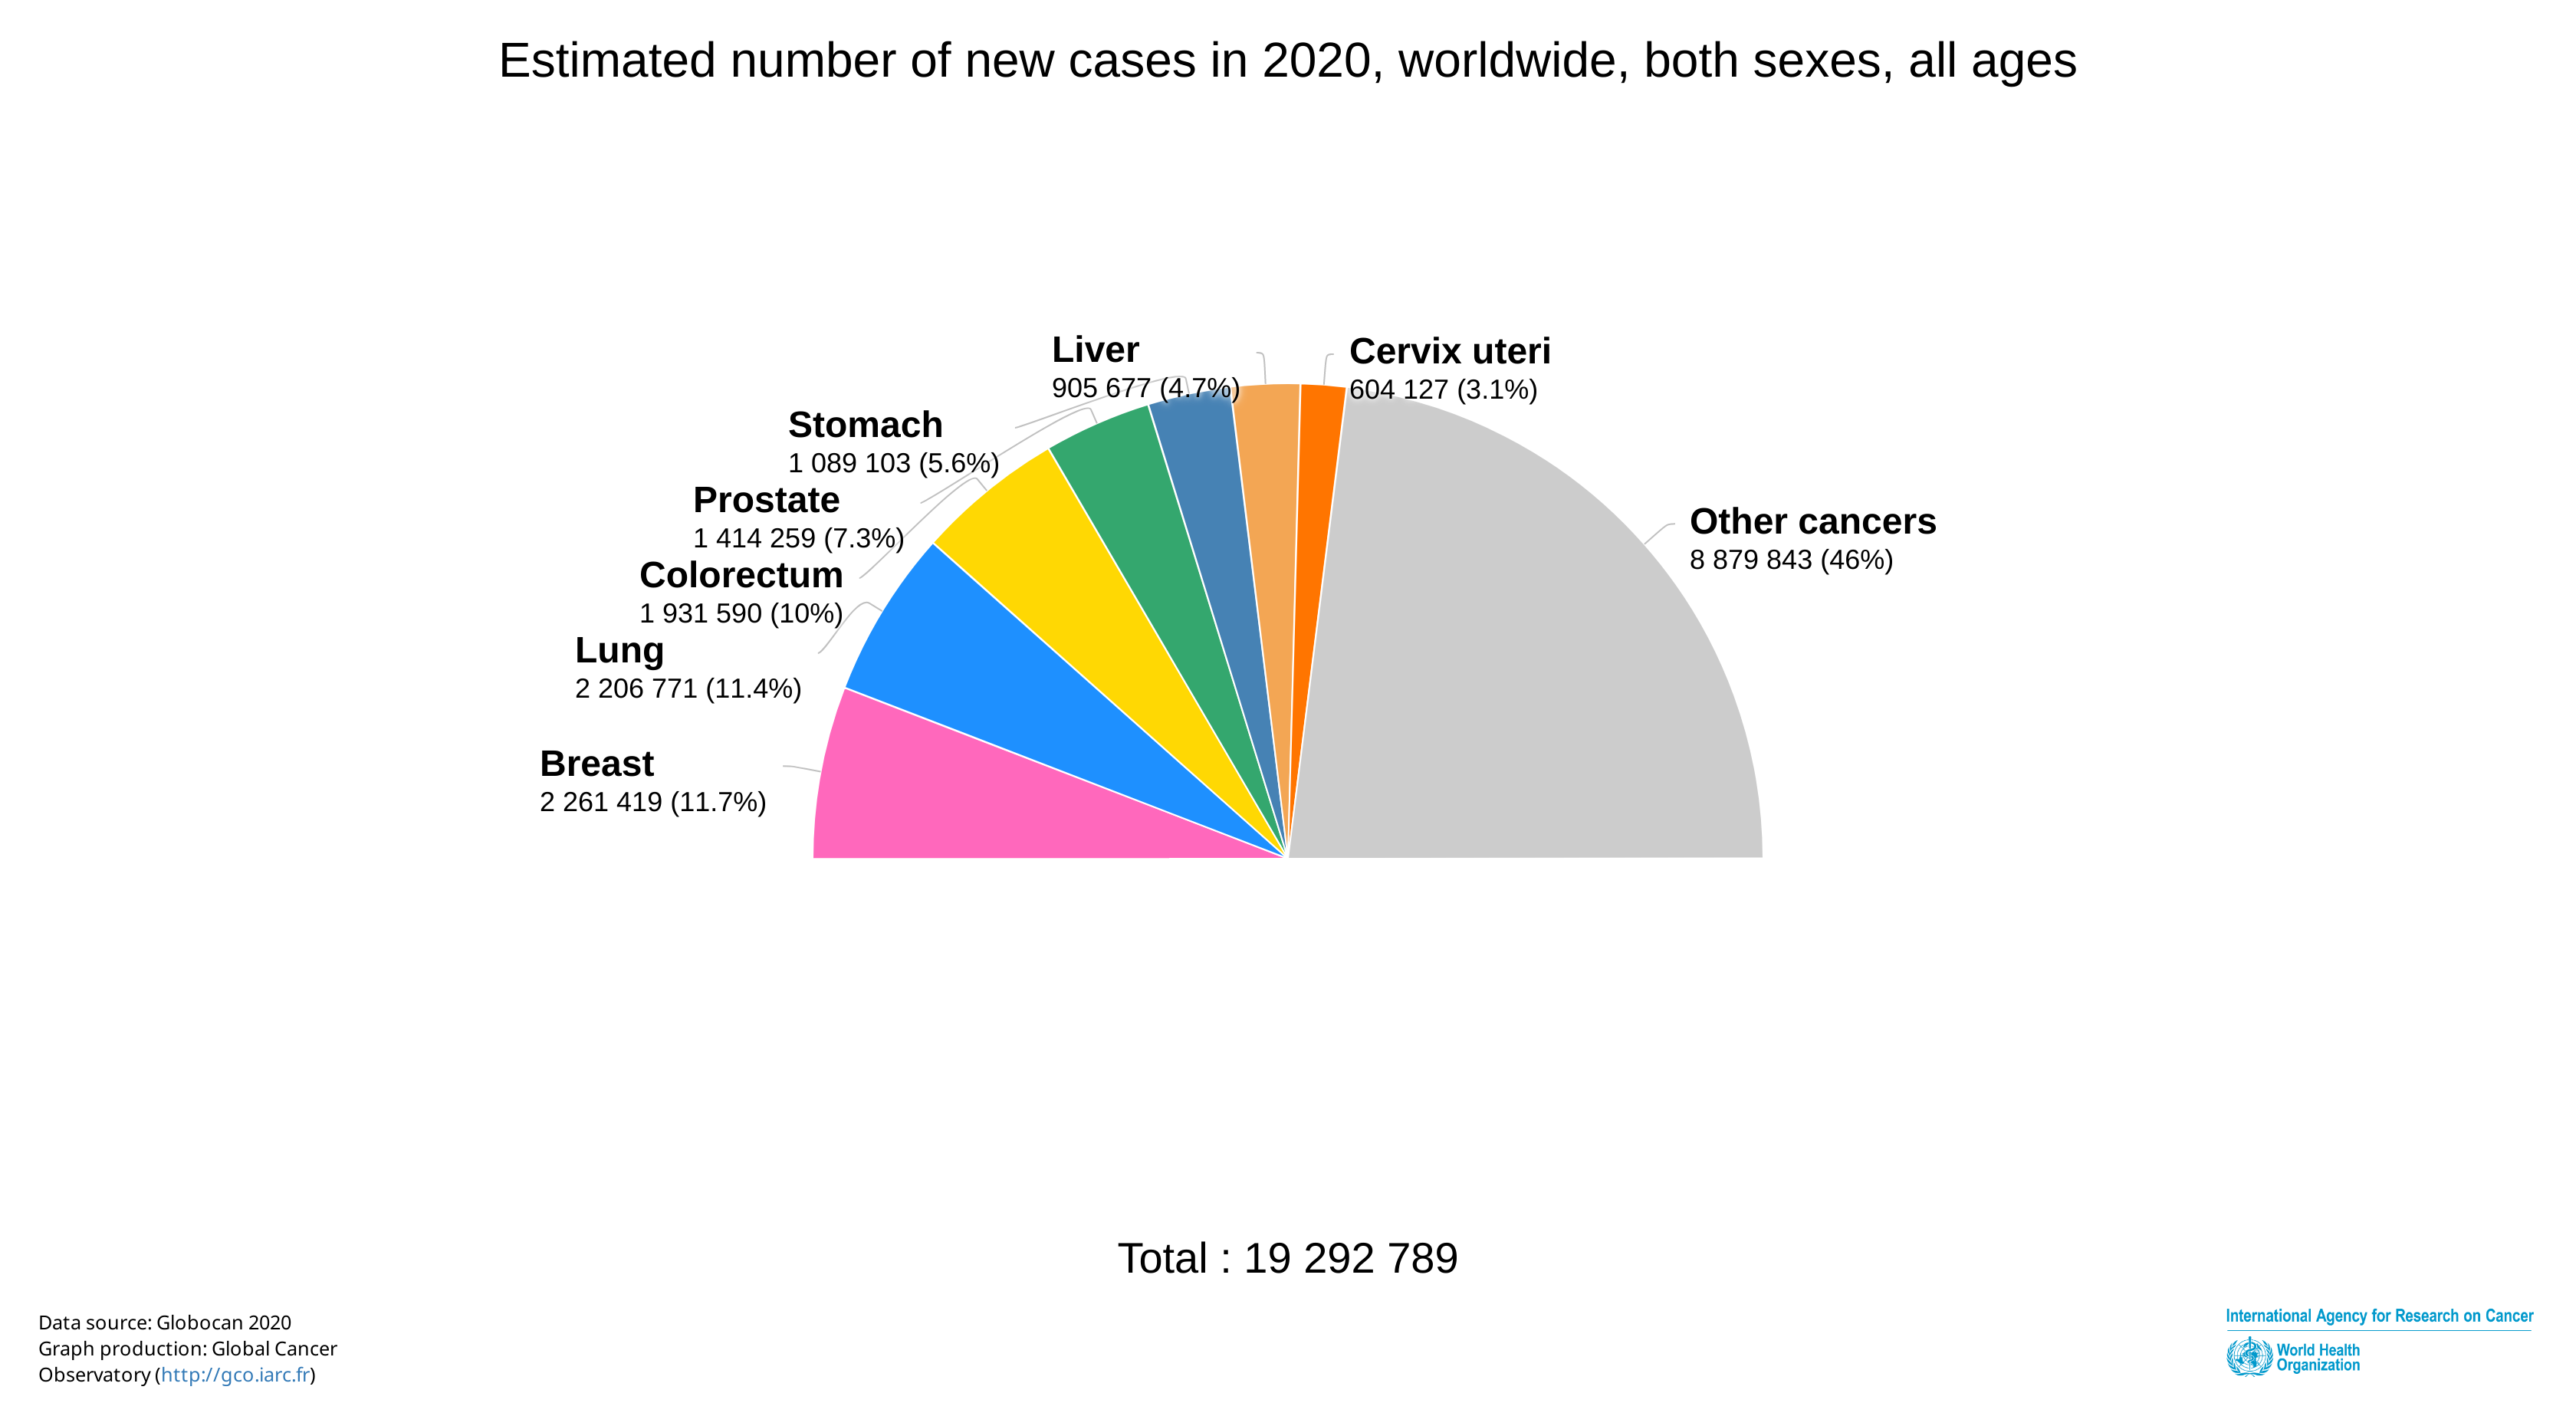
\includegraphics[width=1\textwidth]{images/intro/cancer-proportion.png}
    \centering
    \caption{ \textbf{Estimated number of new cancer cases in 2020, worldwide,
            both sexes, all ages.} According to the GLOBOCAN database,
        the most common cancers in terms of new cases were
        Breast, Lung, Colorectum, Prostate, Stomach, Liver and Cervix uteri.
        In 2020, these 7 cancer types represented more than half of all the
        newly diagnosed cancers.}
    \label{fig:cancer-proportion}
\end{figure}

\begin{figure}[h]
    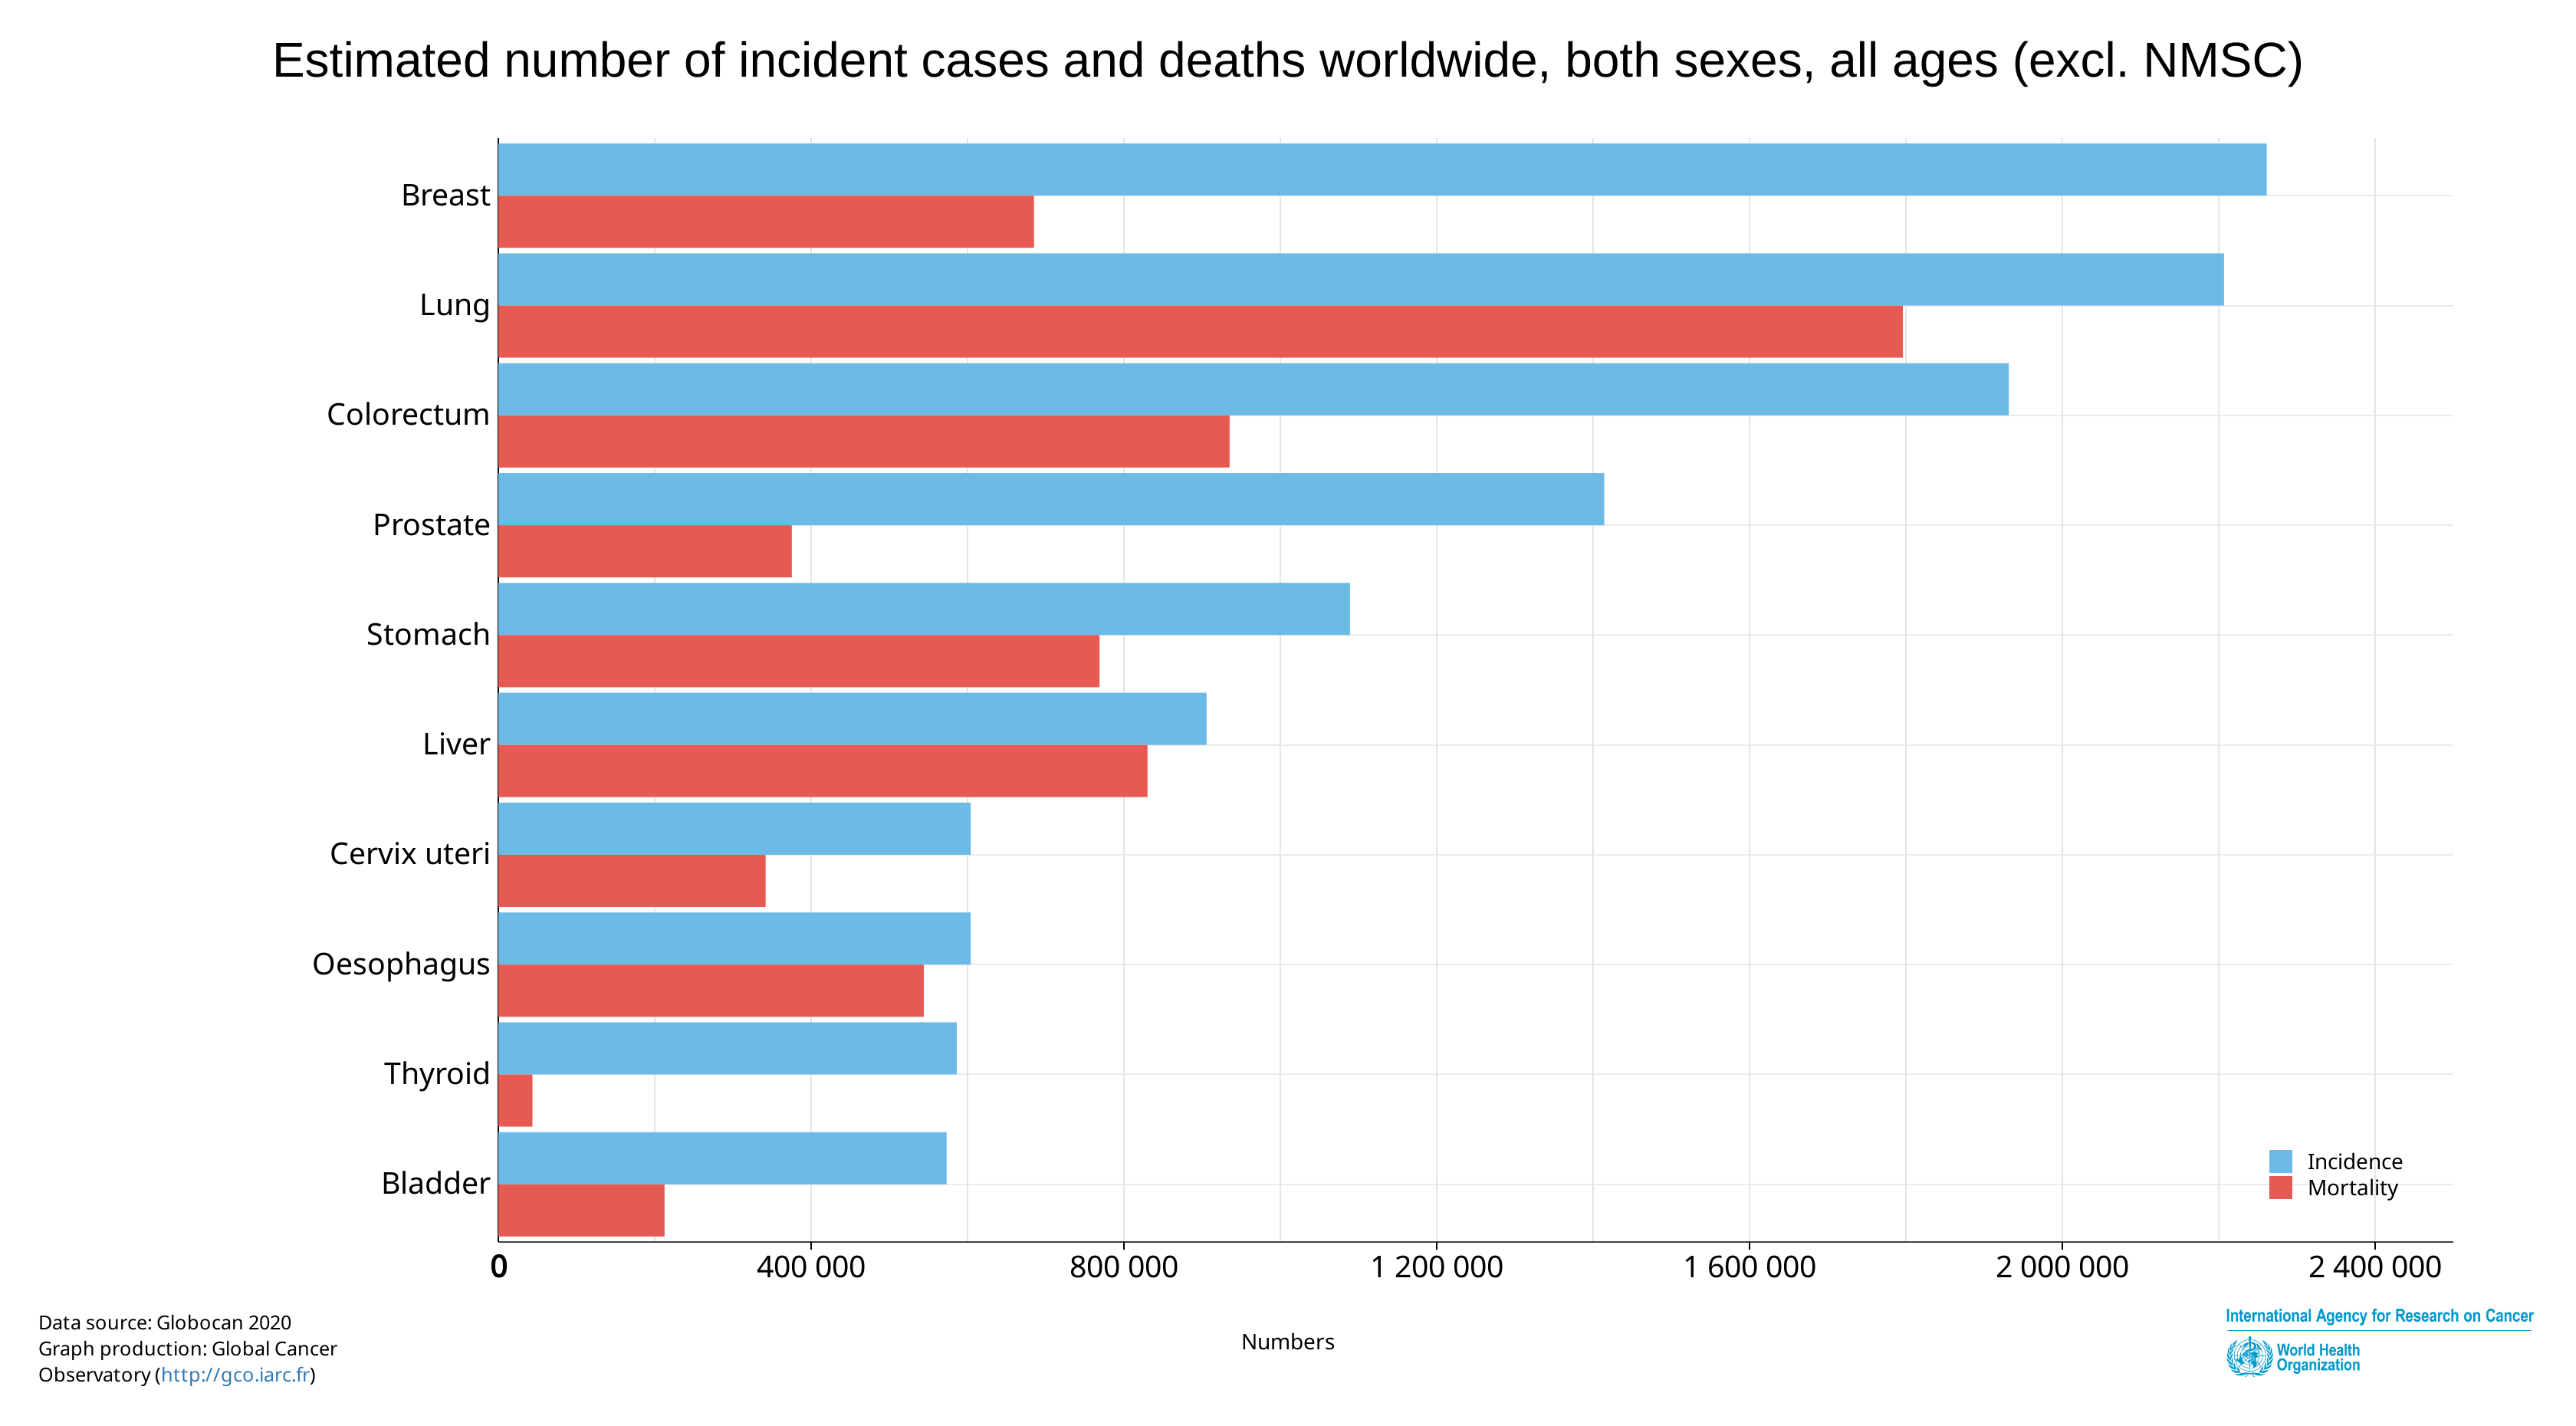
\includegraphics[width=1\textwidth]{images/intro/cancer-incidence-mortality.png}
    \centering
    \caption{ \textbf{Estimated number of incident cases and deaths worldwide,
            both sexes, all ages.} According to the GLOBOCAN database, the most common
        newly diagnosed cancers were Breat, Lung, Colorectum, Prostate, Stomach,
        Liver, Cervix Uteri, Oesophagus, Thyroid and Bladder. The most lethal
        cancers were Lung, Colorectum, Liver, Stomach, Breast, Oesophagus,
        Prostate, Cervix uteri, Bladder and Thyroid. }
    \label{fig:cancer-epidemio}
\end{figure}


\subsection{What causes cancer}

Official and trusted sources like the US
\href{https://www.cancer.gov/about-cancer/understanding/what-is-cancer}{National
    Cancer Institute} or the
\href{https://www.who.int/news-room/fact-sheets/detail/cancer}{\acl{who}} have
online resources explaining what is Cancer and what are its main causes. In the
Cancer disease, some of the body's cells grow uncontrollably and spread to other
parts of the body. Normally, the body's cells grow and multiply when the body
needs them. Old and damaged cells die and are replaced by new cells. This
unwanted cells multiplication may form tumors, which are lumps of tissues. These
tumors can either be cancerous (malignant) or non cancerous (benign). Malignant
tumors can spread into nearby tissues or travel to distant places in the body to
form new tumors, causing metatastic cancer. Cancer is a genetic disease, caused
by changes to genes that control how our cells work. These changes can be caused
by harmful substances in the environment, like chemicals in tobacco smoke or
ultraviolet rays from the sun. They can also come from infections, or be
inherited from our parents. The incidence of cancer rises dramatically with age.
The overall risk accumulation is combined with the tendency for cellular repair
mechanisms to be less effective as a person grows older.

\subsection{Risk factors}

A risk factor is defined as anything that increases the chance of developing a
disease. While it is not possible to know when one will develop cancer, research
shown that certain risk factors do increase the chances of developing cancer.
Some risk factors include expose to chemicals, or certain behaviors like
smoking. Some risk factors cannot be controlled, like age and family history.
The most studied or suspected risk factors for cancer are: age; alcohol;
cancer-causing substances; chronic inflammation; diet; hormones;
immunosuppression; infectious agents; obesity; radiation sunlight; and tobacco.

\subsection{Reducing the cancer burden}

Research estimated that between 30\% and 50\% of cancers can be prevented by
avoiding risk factors and implementing existing evidence-based prevention
strategies. The following recommendations apply to minimize the cancer risk
factors: not using tobacco; maintaining a healthy body weight; eating a healthy
diet, including fruit and vegetables; doing physical activity on a regular
basis; avoiding or reducing consumption of alcohol; getting vaccinated against
HPV and hepatitis B if applicable; avoiding ultraviolet radiation exposure
and/or using sun protection measures; ensuring safe and appropriate use of
radiation in health care (for diagnostic and therapeutic purposes); minimizing
occupational exposure to ionizing radiation; and reducing exposure to outdoor
air pollution and indoor air pollution, including radon. Moreover, an early
detection of cancer and the appropriate treatment and care can also reduce the
cancer burden. As a matter of fact, for many cancers, the probability of being
cured is high with an early diagnosis and the appropriate treatment. When
identified early, the response to treatment is higher, as well as the survival
probability. The treatments are usually less expensive. Significant improvements
can be made in the lives of cancer patients by detecting cancer early and
avoiding delays in care.

\subsection{Cancer treatments}

Every cancer type requires a specific treatment. A proper selection of treatment
depends on both the cancer and the individual being treated. In most cases, the
cancer treatment includes surgery; radiotherapy; and/or systemic therapy such as
chemotherapy, hormonal treatments or targeted biological therapies. The primary
goal of the treatment is either to cure cancer on considerably prolong life.
Besides, maintaining a good quality of life is also important, and can be
achieved with psychosocial and spiritual well-being or palliative care in
terminal stages of cancer. We now explain briefly the the most common treatments
for cancer. A comprehensive list with additional informations is available on
the \href{https://www.cancer.gov/about-cancer/treatment/types}{National
    Cancer Institute website}.

\begin{itemize}
    \item \textbf{Biomarker testing.} Biomarker testing aims at providing
          information on the individual's cancer, by looking for genes, proteins or
          other substances called biomarkers. As some biomarkers affect how cancer
          treatments work, biomarker testing is a way to choose the most suited
          treatment. Biomarker testing is an important part of precision medicine, in
          which the diagnosis and treatment are tailored to the to the genes,
          proteins, and other substances in the patient's body.
    \item \textbf{Chemotherapy.} Chemotherapy is a treatment that uses drugs to
          kill cancer cells. It aims at stopping or slowing down the growth of
          cancer cells. Chemotherapy is used to cure cancer, or ease the
          symptoms. While chemotherapy could be the only treatment received by
          patients, it is often administrated with other cancer treatments,
          based on the cancer type, the spread, and the other health problems
          (called co-morbidities). Chemotherapy treatment often introduces side
          effects such as mouth sores, nausea, hair loss and fatigue, the most
          common side effect. The induced fatigue is such that patients should
          be driven to and from chemotherapy; plan some rest on the day and the
          day after receiving it; and receive help for meals and childcare.
          Chemotherapy can be received during a hospital stay, at home, or an
          outpatient stay (no overnight). The treatment is administered in
          cycles: a period of chemotherapy treatment followed by a period of
          rest.
    \item \textbf{Hormone therapy.} Hormone therapy slows or stops the growth of
          cancer that use hormones to grow, such as some prostate or breast
          cancers. Similarly to chemotherapy, hormone therapy is used to treat
          cancer or reduce its symptoms. Since hormone therapy interferes
          with hormones production, side effects may happen and can be
          different between men and women. Hormone therapy can be taken at
          home, in a doctor's office or in a hospital.
    \item \textbf{Immunotherapy.} Immunotherapy is a treatment that that helps
          the immune system fight cancer. As part of its normal function, the
          immune system detects and destroys abnormal cells and most likely
          prevents or curbs the growth of many cancers. For instance, immune
          cells are sometimes found in and around tumors. These cells, called
          tumor-infiltrating lymphocytes or TILs, are a sign that the immune
          system is responding to the tumor. People whose tumors contain TILs
          often do better than people whose tumors don't contain them. Even
          though the immune system can prevent or slow cancer growth, cancer
          cells have ways to avoid destruction by the immune system.
          Immunotherapy helps the immune system to better act against cancer.
          Several types of immunotherapy are used to treat cancer, including:
          Immune checkpoint inhibitors, T-cell transfer therapy, Monoclonal
          antibodies, Treatment vaccines, Immune system modulators.
          Immunotherapy drugs have been approved to treat many types of cancer.
          However, immunotherapy is not yet as widely used as surgery,
          chemotherapy, or radiation therapy. Immunotherapy can cause side
          effects, many of which happen when the immune system that has been
          revved-up to act against the cancer also acts against healthy cells
          and tissues in your body. You may receive immunotherapy in a doctor's
          office, clinic, or outpatient unit in a hospital.
    \item \textbf{Radiation therapy.} Radiation therapy, also called
          radiotherapy is a treatment that uses high doses of radiations to kill
          cancer cells and shrink tumors. These radiations damage the cells DNA,
          which will eventually stop dividing or die. The cells are not killed
          right away. The treatment may last days or weeks before the cells
          are damaged. At that point, the cells will keep dying for weeks or
          months after the treatment ends. Most of the time, radiotherapy
          is given with other treatments such as surgery, chemotherapy and
          immunotherapy. Radiotherapy may affect nearby healthy cells, thus
          causing side effects.
    \item \textbf{Cancer surgery.} During this procedure, a surgeon removes the
          cancer from the patient body. Many types of cancer are treated with
          surgery, and it works best for solid tumors that are contained in one
          area. The surgery procedure can either remove the whole tumor, or
          part of it. It can also be used to ease symptoms, by removing
          tumors that are causing pain or pressure. The most frequent problems
          that can happen after surgery are pain and infection.

\end{itemize}

\section{Subject definition}

\subsection{Care pathways}

The important developments in oncology treatments seen in the recent years have
improved outcomes for cancer patients. Even though these advances have a
positive impact, they increased the complexity in the delivery of care. To face
the challenges brought by this complexity, care pathways have been introduced.
In the literature, care pathways have been defined as ``a complex intervention
for the mutual decision-making and organisation of care processes for a
well-defined group of patients during a well-defined period''
\cite{vanhaecht_impact_2007}. A care pathway aims at enhancing the quality of
care by improving patient outcomes, increase patient satisfaction and optimizing
the use of resources. Even though the adoption of care pathways is relatively
new for some health services, the concept has long been existing, with first
evidences during the 1950s \cite{schrijvers_care_2012}. In the recent years,
care pathways have gained momentum, with multiple examples of adoption.
Advantages of the care pathways include: faster diagnosis; greater consistency
of care between providers, and better overview for patients; reducing the risk
of errors; and reduction of costs \cite{schrijvers_care_2012}.
The expansion of treatment possibilities can lead to unwarranted variations that
could affect the patients outcome. Adopting pathways is a way to ensure that all
patients receive a consistent treatment, no matter where they are treated.
Moreover, due to the sophistication of oncology care, most patients are treated
by multi-disciplinary team of care providers, sometimes across different
hospital sites. Care coordination is needed between all these providers, to
avoid care gaps and potential errors. Again, pathways can facilitate the
coordination by setting referral points, support data sharing and bring
visibility to into treatment decisions made by all the care providers.
Pathways could also benefit patients before they start their treatment, by
promoting the appropriate use of precision oncology. For instance, by making
sure that patients are not over or under-tested, or that the most optimal
targeted therapeutic is selected based on the patient condition.
Every process that aims at optimizing an operation should be monitored
to identify and address under-performing areas. This is applies to care
pathways as well. Storing and analyzing data related to treated patients during
their patients would allow healthcare teams to evaluate their operations and
optimize their practice patterns. Unwanted care variation could be quickly
discovered and addressed, ultimately preserving patients.

However, due to the growing use of oncology pathways, some challenges
have arisen, notably in the United States. The concerns included the
process being used for pathway development, the administrative burdens on
oncology practices of reporting on pathway adherence, and how to evaluate the
true impact of pathway use on patient health outcomes \cite{zon_american_2016}.
As a result, the American Association of Clinical Oncology (ASCO) articulated
a set of recommendations to improve the development of oncology pathways and
processes. A total of 9 recommendations were proposed for clinical pathway
development and implementation in the oncology setting.
First, a collaborative and national approach should be pursued to reduce
the administrative burdens associated with the non-managed proliferation of
oncology care pathways. Second, the process for oncology pathways development
should be consistent and transparent to all stakeholders. Third, the pathways
should address the full spectrum of cancer care. Fourth, The pathways should
be updated continuously based on scientific knowledge, clinical experience
and patient outcomes. Fifth, physicians should be allowed to easily diverge
from pathways when evidence and patient needs dictate. Sixth, oncology pathways
should be implemented in ways that promote administrative efficiencies for
oncology providers and payers. Seventh, education, research and access to
clinical trials should be promoted to patients during the pathways. Eighth,
robust criteria should be developed to support certifications of oncology
pathways. Lastly, research to understand the impact of pathways on patient
outcomes should be supported.

\subsection{Disparities in care pathways}

There are multiple evidences of disparities in health and care pathways in
the literature, with some due to external factors such as socioeconomic status
or residence location.
% Socioeconomic
Socioeconomic status, reflected by income, education or occupation exacerbates
health problems, including cancer \cite{adler_socioeconomic_2002}. An increase
in mortality has been associated with lower socio-economic status. The cure
rates of children with cancer are much higher in high-income countries than in
the low-income ones \cite{lubega_global_2021}. Indeed, over 85\% of children
with cancer in high-income countries are cured, where only 20\% in many
low-income countries survive the disease. These disparities are caused by
inadequate skilled workforce and health infrastructure. In colorectal cancer,
people from low socioeconomic backgrounds had a higher incidence and mortality
compared to other populations \cite{carethers_causes_2020}. These disparities
might result from differences in exposure to risk factors and limited access to
prevention and treatment resources. In breast cancer, patients with low
socioeconomic status experienced poorer survival rates after diagnosis due to
more advanced cancer stage on presentation and poorer health condition
\cite{silber_disparities_2018}. Research also suggests that outcome disparities
in breast cancer are due to differences in the quality of screening, diagnosis
and treatment \cite{grabinski_disparities_2022}. Overall, the outcome for all
cancer sites combined was higher in poorer countries compared with more affluent
countries. Poorer populations had 13\% higher death rates in men, and 3\% in
women \cite{ward_cancer_2004}. The rate difference between high and low
socioeconomic populations urges the need for research into the mechanisms
causing these disparities. Priority should be given to interventions designed to
reduce disparities by focusing on deprived populations since this is where the
absolute differences in survival are \cite{kish_racial_2014}. A comprehensive
literature review provided a list of disparities in cardio-oncology
\cite{ahmad_disparities_2022}. They classified these disparities into 4 social
determinants categories: race and ethnicity; healthcare access a and quality;
neighborhood and rurality; and economic stability. First race and ethnicity were
shown to have an influence on outcomes, similarly to what has been discussed
earlier. Second, poor healthcare access is linked to delayed care and worse
outcomes. Then rurality was associated to worse outcomes compared to patients in
metropolitan areas. Finally, poor economic stability results in a higher chance
of renouncing to medical care. The research also suggests interventions to
address these disparities, such as targeted policy intervention; increase
diversity in clinical trials; increase access to cardio-oncology care; better
resource allocation; use of social media to promote health literacy; and the
integration of social determinants of health in clinical care delivery. Despite
all these evidences, it seems that the allocation of healthcare resources is
still mostly going to treat diseases, rather than addressing the predisposing
factors of these inequalities \cite{mcginnis_actual_1993}.

% Gender
Finally, gender appears to have an impact on care pathways. For example, men may
have difficulty talking about their symptoms, fearing that it will be perceived
as a sign of weakness; whereas women who require care are more likely to be
neglected \cite{ferrari_gender_2018}. Women with myocardial infarction have a
higher mortality rate than men, and this discrepancy appears to be partially due
to delayed diagnosis and access to appropriate care
\cite{bugiardini_delayed_2017}. Similarly, a pediatric study of kidney
transplantation showed that young girls had less rapid access to transplantation
than young boys. This is partly due to non-medical reasons such as parental and
practitioner behavior regarding organ donation \cite{hogan_j_gender_2016}. For
Head and Neck Cancer (HNC), research found that women had an increased relative
hazard ratio for death versus other causes compared with men. However, they were
less likely to receive intensive chemotherapy and radiotherapy than men. This
might indicate that women in this cohort may be under-treated in clinical
practice and potentially miss the opportunity for their HNC to be aggressively
treated \cite{park_a_undertreatment_2019}. Lastly, women have been
under-represented in clinical trials. Although enrollment of women has increased
over time, it remains lower than the relative proportion in the disease
population \cite{gong_temporal_2019}. Overall, the gender of the patient could
have an impact on the oncology care pathway. Indeed, several studies show that
women's treatment for several types of cancers is suboptimal. This would at
least partially explain why their chances of survival from these diseases are
lower than those of men
\cite{park_a_undertreatment_2019,carter_paulson_e_gender_2009,rose_sex_2016}.
The above examples suggest that patient survival could be improved by taking
gender into consideration in the care pathway. However, at present, gender
differences in the oncology care pathway are barely explored.

\subsection{Cancer in France}

In France, The National Cancer Institute - \acf{inca} is the State agency for
health and scientific expertise in cancer, responsible for coordinating actions
to fight cancer. Created by the Public Health Law of August 9, 2004, it is
placed under the joint supervision of the Ministry of Solidarity and Health on
the one hand, and the Ministry of Higher Education, Research and Innovation on
the other. Since 2003, \acs{inca} produces reports with national recommendations
and measures to mobilize public health actors around prevention, screening,
organization of care, research, support for patients and their families, and
post-cancer care. These reports are called ``cancer plans'', and are supported
at the highest government level in the country by the President. To date, three
cancer plans have been issued, and the last one covered the 2014-2019 period
\cite{buzyn_plan_2014}. This plan is largely focused on inequalities in oncology
care, with objectives to increase knowledge on this issue and address the
problem through specified interventions. These inequalities in cancer care cover
multiple dimensions. Some are territorial; others are social and environmental;
and also depend on other factors such as the age of individuals, their sex or
their genetic characteristics. Inequalities also exist in access to and use of
screening, treatment and therapeutic innovation. This is reflected in particular
in the fact that diagnoses are often made later for disadvantaged social groups,
leading to lower outcomes and more invasive treatments. Similarly, people with
lower incomes or living in deprived communities experience longer delays in
entering the healthcare system, or between the different phases of this system.
Understanding where the inequalities are coming from is a required step to
propose working solutions. The report mention that an information system to
monitor health inequalities was lacking and should be developed. Matching
socio-demographic databases with cancer observation and surveillance tools is
endorsed by the cancer plan. Moreover, the regional health agencies should be
regularly provided with territorialized data on cancer inequalities. Overall,
this last cancer plan provides support for research in cancer inequalities and
population health. The fight against inequalities in cancer care goes far beyond
the field of health. This issue must mobilize actors from the social sector as
well as from education and research. All levels of public action are concerned,
from local to national. This public policy must be built by systematically
integrating the point of view and expertise of patients, especially those from
the least privileged social categories. We should develop solutions to improve
their involvement in the processes and approaches of health democracy.

\subsection{Leveraging medical data in France}

\subsubsection{SNDS database}

Real-life patient data represents an unprecedented and currently underutilized
volume of information, currently under-exploited. In particular, in France, the
Social Security generates a large structured database for administrative
purposes: the National Health Data System - \acf{snds}. The \ac{snds} gathers
complete and up-to-date administrative data on 98\% of the French population.
The exploitation of the \ac{snds}, for research purposes is an exceptional
opportunity to broaden the scope of research in the improvement of care
pathways. Indeed, the substantial number of patients it contains exceeds the
size of all the French cohorts collected in the treatment centers. The \ac{snds}
is one of the largest health databases in the world. It attracts research thanks
to its almost complete coverage of the French population, which makes it
possible to work on the complete care pathway of patients. A major challenge for
the \ac{snds} is to make these data available to promote studies, research or
evaluations of public interest. The \ac{snds} has been effectively used for
research on the following topics: information on health and health care supply;
evaluation of health policies; evaluation of health care expenditure;
information of health professionals on their activity; health monitoring and
safety; research, studies, evaluation and innovation in health. The \ac{snds}
databases contain notably the following data sources: health insurance data;
hospital admissions data; and medical causes of death; Overall, the \ac{snds}
contains more than 3,000 variables; an annual flow of 1.2 billion health
records; 11 million hospital stays; 500 million procedures; and 450 TB of data.
The \ac{snds} contains notably the following data: expenditures and
reimbursements; prescriptions (drugs); medical devices; usage of other services
such as transport; hospital activity and stays; daily allowances and long-term
conditions. The patients characteristics stored in the system are their age, sex
and municipality residence. Patients can be followed throughout their pathways
by a unique identifier. The data in the \ac{snds} are kept for a total of 20
years, then archived for 10 years. However, the \ac{snds} does not contain:
clinical examination results such as imaging or biological data; paraclinical
data such as smoking, blood pressure, BMI; medical consultation reasons; risk
factors such as tobacco, alcohol, or nutrition; drugs delivered during hospital
stays; social data.

\subsubsection{\acs{pmsi} database}

The \acf{pmsi} is a database part of the \ac{snds}, focused on hospital data. It
provides a synthetic and standardized description of the medical activity of
almost every hospital in France. The \ac{pmsi} model was imported from Boston,
MA, from Professor Robert Fetter (Yale University) and the DRG (Diagnosis
Related Groups) models. It was an empirical construction of hospitalization
costs based on several million hospital stays. Initially, in France, it was used
only for descriptive purposes, and not for financial purposes. The \ac{pmsi} was
gradually extended with experiments in both the public and private sectors. The
purpose of these experiments was to study the feasibility of pricing based on
the \ac{pmsi}. Since 2005, it has been used for the implementation of
activity-based pricing (T2A), a new system for remunerating hospitals based on
their activity. The \ac{pmsi} database is used within 4 pans of the hospital
activity: medicine, surgery, and obstetrics (\acs{mco}); psychiatry, follow-up
care; and home hospitalization. We restricted all our analyses to the \acs{mco}
section.

The \ac{pmsi} MCO database is populated with data gathered in the
hospital. For each stay of an inpatient, a standardized discharge summary (RSS)
is produced. This RSS is produced as soon as possible after the patient's
discharge. It must contain a main diagnosis, which is the pathology that
motivated the patient's admission to the medical unit (UM). The RSS can also
contain a related diagnosis, describing the reason for the stay, and associated
diagnoses. The related diagnosis role is to improve the documentary accuracy of
the coding. Diagnoses are coded according to the ICD-10 (International
Classification of Diseases and Use of Health Services No. 10) published by the
\ac{who} and regularly extended by the French Ministry of Health. It may also
contain technical procedures coded according to the CCAM (Common Classification
of Medical Procedures). Each care unit during the stay provides a medical unit
summary (RUM) at the patient's discharge. The RUM contains data concerning the
patient's stay in a given UM: patient's date of birth, gender, municipality,
date of entry into the UM, date of discharge and his medical data such as the
main diagnosis, associated diagnoses and procedures With the synthesis of the
successive RUMs, the standardized discharge summary (RSS) is produced for the
whole stay. The RSS are anonymized and then become anonymous discharge summaries
(RSA) for transmission to the regional health agency (ARS).

\section{Objectives and contributions of the thesis}

\subsection{Objectives}

The objectives of this work is to leverage the real-life patient data to
provide metrics and tools to address the disparities in oncology care pathways,
in France. We chose to address the geographic and socio-demographic disparities
first, and we did not focus on a specific cancer site. The principal data
source used was the \ac{pmsi} database, to access hospitals data and study
the patients care pathways. We restricted the analysis to the year 2018,
and did not study the impact of COVID pandemic in the care pathways. Every
metric and tool that we developed during this thesis will be available for
reuse in other research works.

\subsection{Organization of the thesis}

The following paragraphs describe the chapters of this thesis. First, we
proposed a characterization of every care center is France in terms of
oncology specialization. This oncology label will help physicians, patients,
researchers or public health professionals to better evaluate the hospitals and
their spatial distribution in the country. Second, we computed an oncology
accessibility score, to identify areas where oncology dedicated hospitals
are scarce. Third, we proposed an optimization algorithm to target the hospitals
that should be developed in priority to improve the oncology accessibility.
Fourth, we studied the patients travel from their municipalities of residence
to the hospitals they visit. We developed a travel burden index to not only
measure travel as a distance, but as a combination of distance, duration,
and road sinuosity. We also estimated the carbon footprint of these patients
travel, and simulated a scenario where every patient would travel to the nearest
specialized center. Fifth, we argued that more transparency in oncology care
could benefit patients and help them and their physician to find the most
suited hospital located in a reasonable distance. We built a web application
that lists all the hospitals characteristics, for both patients and physicians.
Finally, we developed an allocation algorithm based on Optimal Transport to
address patients to a nearby and suited hospital. However we only tested this
model on synthetic data, more research is needed to bring it to actual
pathways data.

\subsubsection{Care center characterization}

Countries, such as the UK, USA and Canada, have been implementing a policy of
centralizing the care of patients for many specialized services
\cite{kelly_are_2016}. With such policy, patients are directed to a limited
number of hospitals with higher volumes and more specialized surgeons. There is
evidence that this process will have a positive impact on the health outcomes of
those patients treated in these specialized centres. For instance, centralized
care is beneficial for patients undergoing high-risk procedures, these surgeries
have lower mortality rates when performed by high-volume surgeons
\cite{pekala_centralization_2021,birkmeyer_surgeon_2003,finks_trends_2011,
    hollenbeck_getting_2007,goossens-laan_systematic_2011}. A centralized service
for ovarian cancer may lead to better survival outcomes; evidence from various
other sources suggests that this may also be more cost-effective
\cite{woo_centralisation_2012}. With the rural exodus, the sparsely populated
areas expanded, and several hospitals are serving relatively small populations.
As a result, surgeons operating in these facilities are managing fewer cases of
a given disease. For instance, in the South West of England, surgeons treating
epithelial ovarian cancer were managing fewer than ten cases of ovarian cancer
per year. There is a need to maintain a critical volume of work in order to
sustain surgical expertise \cite{olaitan_surgical_2001}.

Through all these evidences, it is clear that not all the hospitals are equal
for cancer treatment. In France, there are many hospitals that do not have the
same degree of oncology specialization. Hospitals are classified into different
legal categories like public hospitals or private structures, but there is no
indicator to assess the degree of oncology specialization and how large the
hospital is. In this chapter, we first proposed a method to automatically label
all the hospitals in metropolitan France, based on their statistics and
available health services. Lastly, we studied the collaborations between
the hospitals, based on patients who visited multiple hospitals during their
pathways. Through community detection algorithms, we grouped hospitals that
frequently exchange patients together. By adding the oncology specialization
label within the discovered communities, we believe we can propose new
hospital groups that are based on patient real-life data, to improve
collaborations and ultimately benefit the patients.
In this chapter, we first proposed a method to automatically label
all the hospitals in metropolitan France, based on their statistics and
available health services. Lastly, we studied the collaborations between
the hospitals, based on patients who visited multiple hospitals during their
pathways. Through community detection algorithms, we grouped hospitals that
frequently exchange patients together. By adding the oncology specialization
label within the discovered communities, we believe we can propose new
hospital groups that are based on patient real-life data, to improve
collaborations and ultimately benefit the patients.

\subsubsection{Accessibility score}

While a lot of the ongoing research is focusing on finding new cancer
treatments, accessibility to oncology care receives less attention.
Accessibility refers to the relative ease by which services can be reached from
a given location \cite{wang_measurement_2012}. Accessibility can be defined by
spatial factors, determined by where you are; and non-spatial factors,
determined by who you are \cite{khan_integrated_1992}. In what follows, we
restrict accessibility to \acf{sa} and use both terms interchangeably. \ac{sa}
methods assess the availability of supply locations from demand locations,
connected by a travel impedance metric. Supply locations are characterized by
their capacity or quantity of available resource. Similarly, demand locations
are characterized by their population. Such methods have been successfully used
to measure access to healthcare, such as primary care
\cite{guagliardo_spatial_2004} or oncology care
\cite{wang_measurement_2012,zahnd_spatial_2021,alahmadi_spatial_2013} in several
countries including France
\cite{launay_methodology_2019,gusmano_disparities_2014,gao_assessment_2016}.
When measuring accessibility for healthcare, the supply locations are often
physicians locations, whose capacity might be the number of physicians at that
location. Population locations represent where patients live. This could be
the precise address or a municipality. However, while accessibility to primary
care have been described in several studies, there is little work that focused
on oncology care specifically. In what follows, we applied \ac{sa} methods to
quantify the accessibility the oncology care in metropolitan France.
Intuitively, we compute a score for every municipality that measures how easy
it would be for patients living in a given municipality to reach oncology care.

In what follows, we applied \ac{sa} methods to
quantify the accessibility the oncology care in metropolitan France.
Intuitively, we compute a score for every municipality that measures how easy it
would be for patients living in a given municipality to reach oncology care.

\subsubsection{Accessibility optimization}

Uneven distributions of population and health-care providers lead to geographic
disparity in accessibility for patients \cite{wang_why_2020}, illustrated by our
previous results on accessibility. Several methods have been developed to
address these disparities. Location-allocation algorithms
\cite{church_location_1999} can optimize the distribution and supply of health
providers to reduce accessibility disparities. These algorithms seek the optimal
placement of facilities for a desirable objective under certain constraints
\cite{wang_measurement_2012}. For instance, an optimization algorithm  was
developed to improve the healthcare planning in rural China by finding the best
place and capacity for new health facilities \cite{luo_integrating_2014}.
A spatial optimization model was designed to maximize equity in accessibility
to residential care facility in Beijing, China \cite{tao_spatial_2014}. When
optimizing health accessibility, there are two competing goals: equity and
efficiency \cite{krugman_opinion_2013,meyer_equity_2008}. Equity may be defined
as equal access to healthcare for everyone \cite{culyer_equity_1993}. An
efficient situation is when everything has been done to help any person without
harming anyone else \cite{hemenway_optimal_1982}. While some argue that
efficiency should be ad-dressed in priority \cite{hemenway_optimal_1982}, others
agree that equity is a matter of ethical obligation, especially in public health
\cite{fried_rights_1975, oliver_equity_2004}. Regarding efficiency optimization,
the most popular algorithms are p-median, \ac{lscp} and \ac{mclp}. The p-median
algorithm minimizes the weighted sum of distances between users and facilities
\cite{murad_using_2021}. \ac{lscp} minimizes the number of facilities needed to
cover all demand \cite{shavandi_fuzzy_2006}. \ac{lscp} maximizes the demand
covered within a desired distance or time threshold by locating a given number
of facilities \cite{casado_heuristical_2005}. To reach equal access to
healthcare, quadratic programming has been used to  minimize the variance of
accessibility scores defined by the \ac{2sfca} \cite{wang_planning_2013}.
Similarly, a \ac{pso} algorithm was developed to minimize the total square
difference between the accessibility score of each demand location and the
weighted average accessibility score \cite{tao_spatial_2014}. Finally, a
two-step optimization algorithm has been developed to address the dual
objectives of efficiency and equality, by first choosing where to site new
hospitals and then deciding which capacity they should have
\cite{luo_two-step_2017,li_two-step_2017}.

However, most of the previous algorithms seek locations to open new health
facilities. Regarding oncology care, opening new facilities can be very costly
and hard in practice. In this work, we are interested in the case where the
health facilities locations are fixed, and the only lever to improve
accessibility is to increase their capacities.Given a capacity budget, we want
to know which facilities to grow and by how much. We introduce \ac{camion}, an
accessibility optimization algorithm based on \ac{fca} and \ac{lp}. The initial
accessibility score was computed with the \ac{e2sfca} algorithm
\cite{luo_enhanced_2009} but our algorithm can generalize to more \ac{fca}
derivatives. In the following sections, we proposed two approaches for
optimizing the accessibility scores. The first one is an overall optimization,
where we seek to maximize the total accessibility. The second one is a maxi-min
optimization, where we want to maximize the minimum accessibility instead. The
first approach could be seen as efficiency maximization where the second method
aims towards equity. Then, we embedded our results and algorithms into a
web application  called ``oncology-accessibility''. Through this web
application, we let the users run the optimization algorithm with the
parameters they want, and visualize the output on interactive maps and
figures. We believe such an app could benefit the healthcare professionals,
to help addressing the accessibility disparities in the country.

\subsubsection{Patients routes}

Cancer treatment delay is a problem in health systems worldwide, increasing
mortality for many types of cancers \cite{hanna_mortality_2020}, including
breast cancer \cite{caplan_delay_1992, williams_assessment_2015,
    pace_delays_2015}. Distance between patients residence and diagnosing hospitals
is among the factors causing these delays, especially for cancer types that are
hard to diagnose \cite{flytkjaer_virgilsen_cancer_2019}. While accessibility to
healthcare is growing, research found that 8.9\% of the global population (646
million people) could not reach healthcare within one hour if they had access to
motorized transport \cite{weiss_global_2020}. Thus, a non insignificant part of
the population might be exposed to lower prognosis.

The benefits of centralized healthcare have been debated. A centralized approach
often requires patients to travel far away from their home and their local
community hospitals \cite{woo_centralisation_2012}. Patients subject to longer
travels to reach a specialized hospital are likely to be affected by the travel
burden and separation from their social environment \cite{payne_impact_2000}. In
the debate between local versus centralized healthcare provision, there are
evidence of an association between travel distance and health outcomes
\cite{kelly_are_2016}. Unsurprisingly, travel to cancer treatment is
inconvenient for some patients and might even act as a barrier to treatment
\cite{payne_impact_2000}. Research also showed that patients who lived far from
hospitals and had to travel more than 50 miles had a more advanced stage at
diagnosis, lower adherence to encoded treatments, a worse prognosis, and a worse
quality of life \cite{ambroggi_distance_2015}. More research linked travel
burden with lower treatment compliance
\cite{dutta_evaluation_2013,guidry_transportation_1997}. The distance from the
hospital influences the choice of appropriate treatment by cancer patients. In
breast cancer, patients living farther from a radiation treatment facility more
often underwent mastectomy instead of breast conservative surgery
\cite{schroen_impact_2005,celaya_travel_2006,voti_treatment_2006,meden_relationship_2002,nattinger_relationship_2001,boscoe_geographic_2011}
or did not undergo radiotherapy after breast cancer surgery
\cite{satasivam_dilemma_2014,schroen_impact_2005,celaya_travel_2006}. In non
small cell lung cancer, patients were most likely to not undergo potentially
curative surgery if they lived far from a specialist hospital and only attended
a general hospital for their care \cite{tracey_patients_2015}. Moreover, the
necessity for repeated visits for cancer diagnosis and treatment makes distance
an even more important issue for the patient\cite{guidry_transportation_1997}.
However, for hard to diagnose cancer type like rectum or testis cancers,
distance was associated with decreasing odds of advanced disease stage
\cite{virgilsen_travel_2019}. This is possibly due to being treated in more
specialized hospitals. The negative effects of centralized healthcare are even
more pronounced for patients living in rural areas. Indeed, rural cancer
patients face more challenges in receiving care, due to the limited availability
of providers and clinical trials, as well as transportation barriers and
financial issues \cite{charlton_challenges_2015}. There are evidence of poorer
treatments and outcomes for patients living in rural areas. For instance, in
Australia, poorer survival and variations in clinical management have been
reported for breast cancer women living in non metropolitan areas
\cite{dasgupta_variations_2018}. Still in Australia, breast cancer women treated
in a rural hospital had a reduced likelihood of breast conservative surgery
\cite{hall_unequal_2004}.  The hazard of death from ovarian cancer was greater
in women treated at a public general hospital than in women treated at a
gynecological oncology service \cite{tracey_effects_2014}. Contacting a
provincial hospital instead of a university hospital might lead to diagnosis and
treatment delays, which could be improved by a better referral system
\cite{thongsuksai_delay_2000}. In Australia, patients living farther from a
radiotherapy service were more likely to die of rectal cancer, with a 6\% risk
increase for each additional 100km \cite{baade_distance_2011}. In Rwanda, rural
breast cancer patients who lived in the same district as breast cancer hospitals
had a decreased likelihood of system delay \cite{pace_delays_2015}. In Canada,
place of residence seems to influence health outcomes in patients with diffuse
large B-cell lymphoma \cite{lee_effect_2014}. They found that rural and
metropolitan patients had similar survival; however, patients in small and
medium urban areas experienced worse outcomes than those in metropolitan areas.
Thus, rural culture might have a dual effect on health outcomes. On one hand,
distance, transportation, and health services shortage are barriers to
healthcare. On the other hand, rural culture comes with community belonging, and
deeper relationship with health care professionals, which might be beneficial
for some patients \cite{brundisini_chronic_2013}.

Additionally to having a negative impact on patients health, longer travels
participate in global warming due to their \ac{co2} emissions.  The World Health
Organization called climate change the greatest threat to global health in the
21st century, significantly affecting hundreds of millions of people
\cite{change_climate_2015}. The United Nations created the \ac{ipcc} to assess
the science related to climate change and provide governments with scientific
information that they can use to develop climate policies. The health care
sector is an important contributor to \ac{co2} emissions. An international
comparison of health care carbon footprints showed that, on average, the health
carbon footprint in 2014 constituted 5.5\% of the total national carbon
footprint \cite{pichler_international_2019}. Hence, the health sector has a
responsibility to take climate action
\cite{health_care_without_harm_hcwh_global_2021}. Especially since the Paris
Agreement, where countries agreed to cut \ac{ghg} emissions to keep global
warming below 2 degrees Celsius. Today, hospitals are powered by fossile energy
such as coal, oil and gas. Healthcare related travels, and the manufacture and
transport of healthcare products are also major causes of \ac{ghg} emissions.
Ultimately, all health systems will need to reach near zero emissions by 2050,
which can be more cost effective than business as usual. The Lancet Countdown on
health and climate change started to review annually the relation between health
and climate change \cite{watts_2020_2021}. A large share of these carbon
emissions is due to patients journeys
\cite{andrews_carbon_2013,nicolet_what_2022} because most patients travel by car
\cite{forner_carbon_2021}. With centralization of care, patients are encouraged
to be treated in large hospitals for better outcome \cite{eskander_health_2016}.
Such hospitals are in urban areas, and the populations living in rural areas
will have to travel longer to reach these centers, resulting in higher carbon
emissions. In France, few studies have evaluated the ecological impact of cancer
care \cite{guillon_empreinte_2020}. The Shift Project is a French think tank
that works towards a carbon-free economy. As a non-profit organization, they
inform and influence the debate on the energy transition. In 2021, the Shift
Project released a report on how to decarbonize the health care sector in France
\cite{the_shift_project_plan_2021}. They identified that most of the \ac{ghg}
emissions were scope 3 emissions, which are indirect emissions that occur in the
hospitals value chain. Among these emissions, the largest source are
pharmaceuticals and medical device buying, followed by patients and visitors
transportation. The Shift Project states that emissions related to
transportation should be cut by 99\%, through measures like increasing public
transportation and telemedicine. Telemedicine includes all medical practices that
allow patients to be treated remotely from a health facility. It has been used
increasingly around the world, even in oncology where it is sometimes referred
as teleoncology
\cite{mooi_teleoncology_2012,sabesan_are_2014,sabesan_timely_2014,sabesan_medical_2014}.
Teleoncology models have been used to provide access to specialized cancer care
for people in rural, remote and other disadvantaged areas, which minimizes the
access difficulties and disparities \cite{sabesan_telemedicine_2012,
    sabesan_are_2014}. Teleoncology models can also be beneficial in training
medical, nursing, and allied health trainees and staff at rural centers
\cite{sabesan_medical_2014}. Research reported multiple benefits of telemedicine
at every level of care, including education, prevention, diagnosis, treatment,
and monitoring \cite{bertucci_outpatient_2019}. However, besides the expected
benefits, several questions and fears are emerging
\cite{bertucci_outpatient_2019}. First, there is a risk of patient isolation,
due to the absence of in-person meeting. It is also more difficult to build an
atmosphere of trust during remote consultations and the examinations might be of
inferior quality. Finally, digital divide is a major limitation of e-health, as
certain categories of patients do not have access to the internet or to a
smartphone.

In this chapter, we analyzed the travels of cancer patients in metropolitan
France. Our goal was to assess whether the earlier observations on the negative
effects of centralization of care were happening in France. Hence, we first
described the travel duration distribution in metropolitan France, and compared
it with the population densities and the oncology specialization of the visited
hospital. Then, we argued that the negative effects of travel on cancer patients
was not only due to driving distance and duration: the road sinuosity should
also be taken into account. We proposed a travel burden index, which is a
composite indicator based on multiple variables to evaluate how easy it is to go
from a population location to an hospital. Additionally, we estimated the carbon
footprint of cancer patients travels, and compared these numbers across the
different regions. Finally, we ran an optimization algorithm to simulate the
scenario where every patient traveled to the closest hospital, such that the
hospitals capacities were not exceeded. We only considered Breast Cancer
patients as this cancer is relatively frequent, and many hospitals have the
required expertise.

\subsubsection{Transparent healthcare}

% The communications revolution
Over the past few years, there has been a massive change in the way we
communicate and interact with information. The amount of data and content
available to the public keeps increasing, as well as the number of information
delivery platforms. Studies define this phenomenon as ``the communications
revolution'' \cite{viswanath_communications_2012}. Smartphones democratization
and adoption rate are partly responsible for this revolution. Indeed, a large
and growing number of people own a smartphone, enabling them to access
information anytime and anywhere. Through this, there has been a change in how
people access and use information. With the increasing number of media sources,
mass audience is now split into smaller groups who share common characteristics
and interests. Also, the growth of online audience is now far outpacing the
other media. As a benefit of this communication revolution, it is getting easier
to access resources online, even technical resources such as technical reports
and scientific articles. While these materials may not always be intended for a
mainstream audience, their availability offers opportunities for access and
interpretation by different groups.

% Healthcare online resources
The healthcare sector is no exception in this revolution, and health resources
are increasingly available online
\cite{viswanath_science_2005,viswanath_communications_2012}, changing how
patients interact with health providers. Communication has been found to play a
central role in cancer prevention and control. It can provide information on
cancer prevention, monitor lifestyles and health behaviors, promote
participatory decision making during cancer detection, diagnosis, and treatment,
and foster quality of life during survivorship or end of life
\cite{viswanath_communications_2012}. When diagnosed with cancer patients and
their family members lives change radically. They receive treatments and have to
make choices with serious consequences. Such diseases and treatments are
complex, but should be understood before decisions are made. Patients and their
family members should be provided with intelligible and up to date information
on the stage of disease, treatment options and complementary therapies
\cite{butow_dynamics_1997,cassileth_information_1980}.
Multiple benefits of bringing more information to the patients have been
reported. Involving cancer patients in decision-making on their pathways
improves their satisfaction and quality of life, compliance with treatment and
their ability to manage symptoms
\cite{johnson_effects_1982,hack_feasibility_1999,mohide_randomised_1996,mcpherson_effective_2001,
    sheabudgell_information_2014,huchcroft_testing_1984,cegala_patient_2003,viswanath_science_2005}.
Moreover, medically related education interventions are most effective when they
are tailored to patients' individual needs, especially for cancer patients
\cite{cegala_patient_2003}. Through all these benefits, it is clear that
monitoring patient information seeking experiences over time is important
\cite{finney_rutten_cancer-related_2016}.

% Patients information seeking
As a matter of fact, patients are often seeking information during their
pathways. In the United States of America, a survey from the Health Information
National Trends (HINTS) \cite{hesse_trust_2005} measured online health
activities, levels of trust, and source preference for 6,369 people. They
observed that physicians remained the most trusted source of information,
despite an increasing number of people looking for information online.
However, there is increasing evidence in the literature that patients are often
not satisfied with the information they received. Some reported to lack
information on their disease and its consequences
\cite{mcpherson_effective_2001}, while others forget or misunderstand the
information conveyed \cite{ley_communicating_1988,hogbin_getting_1989}. The
interaction with their physician has also been cited as a major cause of
dissatisfaction \cite{stewart_effective_1995,bartlett_effects_1984} at all
stages of illness \cite{higginson_palliative_1990}. Patients reported
insufficient time spent on communication during the clinical encounter and
physicians inability to keep up with the most current information and advances
in cancer care \cite{anderson_impact_2003}. Some patients reported incorrect
diagnosis, or not receiving the most up-to-date cancer information from their
physician, especially for rare cancers \cite{dolce_internet_2011}. Patients who
need health information but experience difficulties have been found at risk of
experiencing poorer psychosocial health \cite{arora_barriers_2002}.
A Canadian study surveyed patients attending appointments at follow-up cancer
clinics in Calgary, Alberta \cite{sheabudgell_information_2014} between 2011 and
2012. They approached 648 patients and obtained responses from 411 one of them.
The study aimed at: identifying information needs of patients when meeting their
physician for a follow-up; listing patients preferences on how to receive
information. Here are the results they gathered regarding information seeking
patterns. The most frequently reported source of information was the Internet
(57.4\%); health provider (32.6\%), brochures or pamphlets (25.1\%), and cancer
organizations (24.3\%). The most frequently reported types of information sought
included information about a specific type of cancer (43.1\%), treatment or
cures for cancer (29.4\%), prognosis or recovery from cancer (29.0\%), and
prevention of cancer (27.0\%). The least frequently reported types of cancer
information sought included where to get medical care (3.4\%), paying for
medical care or insurance (4.6\%), and cancer organizations (5.4\%). Regarding
trust, the physician or health care provider was largely the most trusted source
of information, followed by Internet, and family and friends. The least trusted
sources of information included radio, newspaper, and television.
More evidence is reported on the use of the internet for health information
retrieval
\cite{chen_impact_2001,pereira_internet_2000,ziebland_how_2004,dolce_internet_2011}.
For instance, an online questionnaire was administered to participants of
cancer-related communities hosted by the Association of Cancer Online Resources
(ACOR) \cite{dolce_internet_2011}. As a result, 488 participants shared their
personal experiences on why and how they accessed online health resources.
Participants who experienced a lack of informational support related to
procedures found blogs and testimonies online that helped them to know what to
expect from a physical and emotional perspective. Moreover, for rare diseases,
physicians might actually benefit from patients looking from additional
information online, as it could bring additional knowledge to them, and even
change their plans for care. Aware patients can also challenge their physicians
by asking meaningful questions and participate in the tailoring of their
treatment plans. Finally, online communities allowed patients to identify
physicians with a proven track record in cancer care. They endorsed care
providers who took the time to answer questions, as well as specialists from
major cancer centers, that brought superior care which led to better outcome.
Indeed, \ac{gp} play a crucial role in early cancer detection because the
majority of cancer patients initially consult their \ac{gp} with symptoms.
Therefore, the actions taken by the \ac{gp} upon the patient's symptom
presentation may considerably affect the cancer trajectory
\cite{flytkjaer_virgilsen_cancer_2019}. To sum up, the increased usage of the
Internet by cancer patients puts new demands on health care professionals.
Patients need advice about how to find reliable and credible web sites and also
help with authenticating and interpreting the information they find
\cite{carlsson_cancer_2009}.

% Bringing transparency in cancer surgery
While patients are looking for informations on their symptoms, diseases and
treatments, it would be crucial for them to know better about their physician's
ability, especially for cancer surgery. In cancer care, surgery is one of the
most important part of the treatment, and is directly linked to the surgeon
ability.
Surgeon and hospital-related factors have been found to be direct predictors of
outcome in colorectal cancer surgery \cite{renzulli_influence_2006,
    bonati_surgeon_2021}. In breast cancer, patients managed by high-volume surgeons
were more likely to have breast-conserving surgery (BCS) than those managed by
low-volume surgeons \cite{mcdermott_surgeon_2013}. Moreover, breast cancer
patients who receive treatment from experienced and specialized surgeons are
more likely to receive the standard sentinel lymph node biopsy
\cite{yen_surgeon_2014}. The surgeon's expertise and learning curve is directly
related to the patient's outcome \cite{renzulli_learning_2005}. A low surgeon or
hospital caseload may be compensated by intensified supervision or by improved
training and teaching \cite{bonati_surgeon_2021}. From all these findings, it is
questioned whether surgeons should have an ethical obligation to inform patients
of their surgical volume and outcomes \cite{glaser_surgeon_2019}. One way to
monitor the surgeons abilities is the use of quality indicators, which have been
developed in high income countries and contributed to improved quality of care
and patient outcomes over time \cite{nietz_quality_2020}.
With these evidences of healthcare information needs, we developed Healthcare
Network, a web application that lists every hospital in France, and displays key
statistics on them. The application is directed to either health professionals
or patients. Health professionals might use it to gain insights about specific
hospitals, and look for the best place to send their patients when they lack
expertise. Patients could learn more about the hospital they have been sent to,
check the care quality or surgery volume.

\subsubsection{\acl{simca}}

% Background
In a very broad range of applications -- many of them being led by e-commerce
leaders (Amazon \cite{linden_amazoncom_2003}, Netflix \cite{koren_matrix_2009})
-- recommendation algorithms have been increasingly used over the past decade.
These algorithms are capable of showing users a personalized selection of items
they may like, based on their interests and user behavior.

% Problem we want to solve
Up to now, the predictions are built upon user-item affinity scores (e.g.,
user/movie ratings) which are obtained from high-dimensional embeddings of items
and users. While these approaches work for most e-commerce applications, there
are other natural settings in which more attributes should be considered in the
recommendation process. For instance, item capacity constraints are of paramount
importance in location or route recommendation, where recommending the same item
to every user could lead to congestion and significantly deteriorate  user
experience \cite{christakopoulou_recommendation_2017}. Moreover, in the case of
location recommendation, travel distance is also a key factor: the user's choice
is often the result of a trade-off between affinity and proximity
\cite{zhao_survey_2016}. In the healthcare sector, patients are usually
addressed to an hospital by their general practitioner -- or by word of mouth.
Since the choice of hospital and practitioner may be critical, an important
issue is to make sure that patients are routed to the best place possible --
namely to a nearby and adapted structure, without capacity saturation. Benefits
of such systems have been documented in the literature. For instance, an
application similar to Google Maps for guiding patients to different care
centers in a multi-site hospital reduced patient travel time
\cite{mandel_optimizing_2018}. Another research proposed a method to select the
optimal care center using several criteria such as geographic accessibility and
service quality. In particular, transportation networks such as high-speed lines
and highways are taken into account in the center selection
\cite{jia_selecting_2014}.

% Proposed method, contributions and paper organization
In this work, we study the recommendation problem in the setting where
affinities between users and items are based both on their embeddings embeddings
in a latent space and on their geographical distance in their underlying
euclidean space (e.g., $\mathbb{R}^2$), together with item capacity constraints.
Upon the observation of an optimal allocation, user embeddings, items
capacities, and their positions in the euclidean space, our aim is to recover
item embeddings in the latent space; doing so, we are then able to use this
estimate e.g. in order to predict future allocations. Our contributions are as
follows:

\begin{itemize}
    \item[$(i)$] we propose an algorithm based on matrix factorization enhanced
        with optimal transport steps to model user-item affinities and learn item
        embeddings from observed data;
    \item[$(ii)$] we then illustrate and discuss the results of such an approach
        for hospital recommendation on synthetic data.
\end{itemize}

After reviewing related work, we formally define the problem in mathematical
terms, we describe our algorithm for \ac{simca} and give theoretical guarantees
on its convergence. We then illustrate our method for the hospital
recommendation problem on synthetic data, discussing the results as well as the
choice of parameters.
